%% LaTeX template for BSc Computing for Games final year project dissertations
%% by Edward Powley
%% Games Academy, Falmouth University, UK

%% Based on:
%% bare_jrnl.tex
%% V1.4b
%% 2015/08/26
%% by Michael Shell
%% see http://www.michaelshell.org/
%% for current contact information.
%%
%% This is a skeleton file demonstrating the use of IEEEtran.cls
%% (requires IEEEtran.cls version 1.8b or later) with an IEEE
%% journal paper.
%%
%% Support sites:
%% http://www.michaelshell.org/tex/ieeetran/
%% http://www.ctan.org/pkg/ieeetran
%% and
%% http://www.ieee.org/

%%*************************************************************************
%% Legal Notice:
%% This code is offered as-is without any warranty either expressed or
%% implied; without even the implied warranty of MERCHANTABILITY or
%% FITNESS FOR A PARTICULAR PURPOSE! 
%% User assumes all risk.
%% In no event shall the IEEE or any contributor to this code be liable for
%% any damages or losses, including, but not limited to, incidental,
%% consequential, or any other damages, resulting from the use or misuse
%% of any information contained here.
%%
%% All comments are the opinions of their respective authors and are not
%% necessarily endorsed by the IEEE.
%%
%% This work is distributed under the LaTeX Project Public License (LPPL)
%% ( http://www.latex-project.org/ ) version 1.3, and may be freely used,
%% distributed and modified. A copy of the LPPL, version 1.3, is included
%% in the base LaTeX documentation of all distributions of LaTeX released
%% 2003/12/01 or later.
%% Retain all contribution notices and credits.
%% ** Modified files should be clearly indicated as such, including  **
%% ** renaming them and changing author support contact information. **
%%*************************************************************************


\documentclass[journal]{IEEEtran}

\usepackage{graphicx}
% Insert additional usepackage commands here
\usepackage[hyphens]{url} % <===========================================
\usepackage[hidelinks]{hyperref} % Allows clickable reference lists
\usepackage[none]{hyphenat} %Stops breaking up words in table
\usepackage{cite}
\usepackage{listings}

\begin{document}
%
% paper title
% Titles are generally capitalized except for words such as a, an, and, as,
% at, but, by, for, in, nor, of, on, or, the, to and up, which are usually
% not capitalized unless they are the first or last word of the title.
% Linebreaks \\ can be used within to get better formatting as desired.
% Do not put math or special symbols in the title.
\title{ How Will the Introduction of a Mixed-Initiative Component that Predict User Requirements Affect the Size and Speed of the Levels Created?}
%
%
% author name

\author{Tristan Barlow-Griffin}

% The paper headers -- please do not change these, but uncomment one of them as appropriate
% Uncomment this one for COMP320
\markboth{COMP320: Research Review and Proposal}{COMP320: Research Review and Proposal}
% Uncomment this one for COMP360
% \markboth{COMP360: Dissertation}{COMP360: Dissertation}

% make the title area
\maketitle

% As a general rule, do not put math, special symbols or citations
% in the abstract or keywords.
\begin{abstract}
The abstract goes here.
\end{abstract}




\markboth{COMP320: Research Review and Proposal}{COMP320: Research Review and Proposal}

\section{Introduction} \label{intro}
\IEEEPARstart{T}{his} research project will look whether a prototyping tool that predict user requirements will increase the size and speed of levels designed. A prototype is the initial design of an object \cite{prototype}. The prototyping phase of a project is used to quickly test certain aspect of a products' design so the designer can identify and clear up any problems\cite{budde1992prototyping}.Fullerton \textit{et all} \cite[p.~150]{fullerton2004game} state there are two kinds of prototyping in games: Physical and Software prototypes. Since this book was published back in 2004, the accessibility of software tools to help prototyping has increased. The author of \cite[p.~164]{fullerton2004game} also describes level editors as a good way to prototype levels. \textit{Unreal Engine 4} (UE4) implement their own version of a level editor. Within this editor the designers can create basic geometry scaling them to fit their needs as well as addition custom meshes and programmable objects.

This paper looks to build upon  a normal level editor by adding a Mixed-Initiative component that will predict the users requirements. The component will aim to reduce the time it takes to produce a level prototype. As discussed above the prototyping phase is meant to test a design, the less time and resources required to produce an artefact that can demonstrate the proposed design the better. Beyond the benefit of saving time, the less time a designer puts into a particular design the less attached to the design they become. When collaborating in a group, differing opinions can cause different constraints to be set on the design of a level. While a given design may satisfy the original designers set constraints, the prototype may have to be discarded as it did not meet the other requirements set by the team. Identifying and discarding concepts early in development can save a lot of time and energy \cite[p.489]{stempfle1999thinking} and arguable may reduce the negative impacts to interpersonal relations that idea dismissal may have. 

\section{Related Work}
The main focus of this literature review will be on prediction methods. For the research into prediction methods the scope went beyond just game design as their were limited cases of prediction methods to be found. To discover whether mixed-initiative tools really have a place in level design the selection of the prediction method must be optimal. When researching prediction methods scoping considerations have been taken into account. Some prediction methods have been the centre of studies with far more resources than this project. Prediction methods referenced are not cutting edge in the field.  The definition of mixed-initiative used in this paper will also be defined in  Section~\ref{MI}. The category of mixed-initiative tool to be used defined as by \cite{liapis2016mixed} definition, this definition is used by other researchers \cite{alvarez2018fostering} . This literature review will also look at mixed-initiative editors already published using their results to refine the design of interface. 

\subsection{Mixed-initiative} \label{MI}
The term mixed-initiative was first introduced by Jaime R \cite{carbonell1970mixed}.
It describes a process where by a computer and a human designer work together to achieve a goal. The first instance of mixed-initiative was a tool to help students learn the English language. The uses of mixed-initiative tools has greatly expanded since 1970 and have been described as a backbone tool for designers \cite{alvarez2018fostering}.

The two broad categories that MI tools can be grouped into are: Interactive evolution and Computer-aided design \cite{liapis2016mixed}. 
\begin{itemize}
    \item \textit{Interactive evolution}(IE) is where the designer has the idea and the computer helps them realise it. The computers role is to evaluate the humans design, presenting alternative solutions if any constraints are broken. 
    
    \item \textit{Computer-aided design} (CAD) is where the computer generates the content, but does not evaluate the quality of the produced work. Instead, a human designer will evaluate the work and use the evaluations to move towards a more desirable product space.
\end{itemize}

The field of procedural content generation has advanced significantly \cite{van2013designing}, these uses of CAD are ever increasing as publishers seek to lower costs of production\cite{doherty2005mixed, font2016constrained}. As the field grows in popularity the research into it grows also. Using CAD may increase the quantity and variation of levels produced ensuring replayability \cite{karavolos2015mixed}. These algorithms are the topics of large research papers, with in depth analysis to how re-playable they make a game. From reading within the field it can be argued that all of the instances of CAD require a programmer of modest ability to implement the generation algorithms. As a result, when prototyping levels, generations algorithms are not usually employed unless a programmer can be spared. As discussed above in Section~\ref{intro} the shorter time prototyping the better. This is where an IE tool may prove to be more helpful than CAD algorithm. Even with parameters available the core of the creative process will be on the computer. Within an IE environment  the core of the creative process relies on the human designer. As the main creative driver the human has the most input, with the computer ideally providing supplementary support. It can be argued as the constraints are determined more by the human the size of the possible output space will be larger. Yanakakis \textit{et al} \cite{yannakakis2014mixed} claim that CAD examples like PCG limit the designers intentions as they follow their own algorithms which ideally should have a set of designer centric parameters as their only form of control \cite{doran2010controlled}.

\subsection{Mixed-Initiative Level Designers } \label{UI}
A user interface should be intuitive to use and not require any additional help systems \cite{oppermann2002user}.Liapis  \textit{et al} \cite{liapis2013sentient} aim to achieve this by  creating a design tool that allows users to create levels using a low resolution graphical interface. Figure~\ref{Sketchbook} shows their interface used to design levels for a strategy game. The designer can place tiles on the map which will colour in the given tile with the placed tiles colour. During a placement the tool will test for the maps playability, checking to see if placing the current tile will break any of the games constraints.  The Sentient sketchbook also provides alternative viewing modes, examples of these alternate viewing models can be seen in Figure~\ref{Sketchbook2}.  There is no mention in the study how often these tools were used, it can be argued that the virtualisation while nice, just added needlessly to skill required to use this tool effectively.

\begin{figure}[h]
	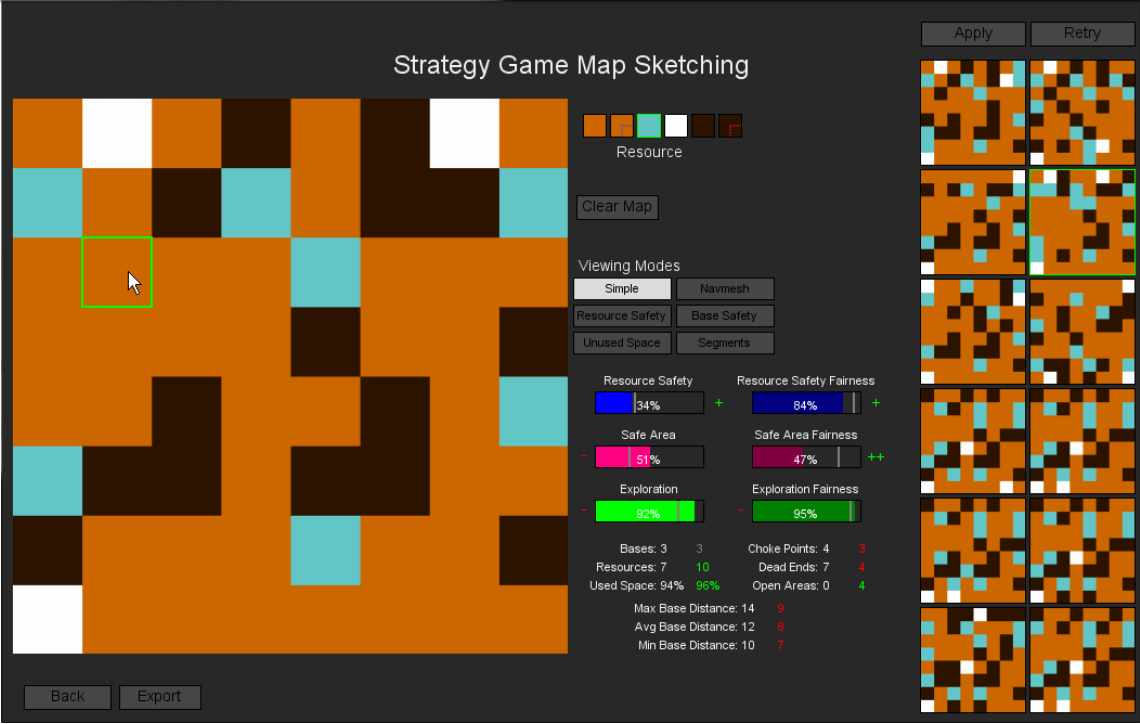
\includegraphics[width=1.0\linewidth]{SentientSketchbook.PNG}
	\caption{A. Liapis \textit{et al} Sentient Sketchbook during a design session ~\cite{liapis2013sentient}.}
	\label{Sketchbook}
\end{figure} 

\begin{figure}[h]
	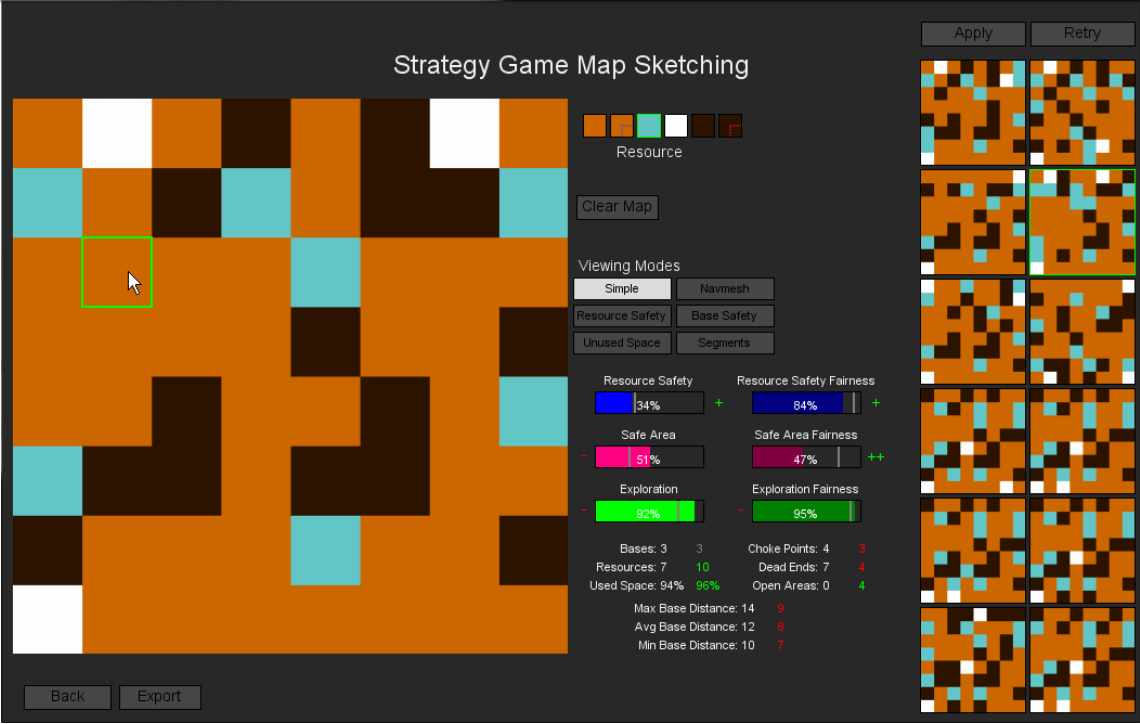
\includegraphics[width=1.0\linewidth]{SentientSketchbook.PNG}
	\caption{A. Liapis \textit{et al} Sentient Sketchbook Different viewing modes ~\cite{liapis2013sentient}.}
	\label{Sketchbook2}
\end{figure} 

Horvitz \textit{et al} \cite{horvitz1999principles} propose 12 critical factors to take into consideration when making a mixed-initiative user interface. While Horvitz \textit{et al} \cite{horvitz1999principles}  focuses on an mixed-initiative assistant for Microsoft Outlook (emailing software) it can be argued that some of these factors are relevant for level design .  The first factor that is listed is that a MI tool needs to add significant value through the automation of services. An Examples of a services automated by emailing assistant is the sorting of a users emails into different categories.   Within in the context of \cite{liapis2013sentient}  they satisfy \cite{horvitz1999principles} first critical factor by allowing the computer to automate some of the map design services like checking for broken game constraints. Liapis \textit{et al} \cite{liapis2013sentient} also allow their algorithm take on a creative role all be it based on an original human designed map. Within this project the focus will not be on the creative aspect as the definition of creativity is hard to for a computer to understand \cite{jordanous2010defining}. It can be argued that an MI tool could not consistently add value as it can not understand the designers creative vision. 

Another factor raised by \cite{horvitz1999principles} is that an MI tool must consider minimizing the costs of poor guesses about the users goals. Even with an extensive history of user goals, novel goals might be implemented during this time the system will benefit from the understanding it cannot predict what the user is trying to accomplish.  Some authors find value in these missed guesses and even seek to find novelty search spaces \cite{liapis2013sentient}. Other authors \cite{liapis2016can,alvarez2018fostering, yannakakis2014mixed} claim these kind of mistakes can foster creativity and alternate suggestions that do not aim to predict the user can be beneficial. On the right hand side of Figure~\ref{Sketchbook} is where the guessing algorithms results are shown. Clicking retry will quickly remove the selected map and create a new one. 




\subsection{Prediction Methods} \label{prediction}
Predictive texting increases the average message length users send to each other \cite{ling2005length} as well as the speed the words are written \cite{dunlop2000predictive}. The same theory may apply to game design. If patterns to a users game design are established, an AI system may be able to assist in design. However, the principle with working with predictive texting is different to that of game design.

The researchers of \cite{chipalkatty2013less} tested alternate methods for predicting human input so as to abstract the low-level movements of the robots the humans were controlling. They built on the idea that humans are good for high-level abstract tasks, but an AI agent was much better at performing low-level repetitive control tasks. They also found that when trying to predict the input the human would do next, trying to identify patterns in a history of inputs was far less successful at predicting the humans intention than just using the last input given by the human. Instead of using current human inputs, \cite{bhatia2016targeted} used the history of the humans social media page to predict the users interests. Perhaps if the authors of \cite{chipalkatty2013less} had looked less at the input history of the human and instead focused on grouping inputs together to create larger actions. Similar, to how modern day phones often predict entire sentences rather than just single words.



\section{Proposal}
The experiment proposed in this studies involves...

\bibliographystyle{IEEEtran}
\bibliography{references}

% Appendices

\appendices
\section{First appendix}
Appendices are optional. Delete or comment out this part if you do not need them.

% that's all folks
\end{document}
